%%%%%%%%%%%%%%%%%%%%%%%%%%%%%%%%%%%%%%%%%%%%%%%%%%%%%%%%%%%%%%%%%%%%%%
\section{\label{sec:install}Installation}
%%%%%%%%%%%%%%%%%%%%%%%%%%%%%%%%%%%%%%%%%%%%%%%%%%%%%%%%%%%%%%%%%%%%%%

This section contains the instructions for installing Condor.
The installation will have a default configuration that can
be customized.
Sections of the manual that follow this one explain customization.

Read this entire section before starting installation.

Please read the copyright and disclaimer information in 
section~\ref{sec:license} on
page~\pageref{sec:license} of the manual.
Installation and
use of Condor is acknowledgment that you have read and agree to the
terms.

%%%%%%%%%%%%%%%%%%%%%%%%%%%%%%%%%%%%%%%%%%%%%%%%%%%%%%%%%%%%%%%%%%%%%%
\subsection{\label{sec:pre-install-procedure}
Obtaining Condor}
%%%%%%%%%%%%%%%%%%%%%%%%%%%%%%%%%%%%%%%%%%%%%%%%%%%%%%%%%%%%%%%%%%%%%%
\index{installation!download}
\index{Unix installation!download}
\index{download}
The first step to installing Condor is to download it from the Condor
web site, \URL{http://www.cs.wisc.edu/condor}.
The downloads are available from the downloads page,
at \URL{http://www.cs.wisc.edu/condor/downloads/}.

The platform-dependent Condor files are currently available from two sites.
The main site is at the University of Wisconsin--Madison,
Madison, Wisconsin, USA.
A second site is the Istituto Nazionale di Fisica Nucleare Sezione di
Bologna, Bologna, Italy.
Please choose the site nearest to you.

Make note of the location of where you download the binary into.

The Condor binary distribution is packaged in the following files
and directories:

\begin{description}
\item[\File{DOC}] directions on where to find Condor documentation
\item[\File{INSTALL}] these installation directions
\item[\File{LICENSE.TXT}] the licensing agreement.
                  By installing Condor, you agree to the contents of
		  this file
\item[\File{README}] general information
\item[\File{condor\_install}] the Perl script used to install and
                  configure Condor
\item[\File{examples}] directory containing C, Fortran and C++ example
		  programs to run with Condor
\item[\File{bin}] directory which contains the distribution Condor
		  user programs.
\item[\File{sbin}] directory which contains the distribution Condor
		  system programs.
\item[\File{etc}] directory which contains the distribution Condor
		  configuration data.
\item[\File{lib}] directory which contains the distribution Condor
		  libraries.
\item[\File{libexec}] directory which contains the distribution Condor
		  programs that are only used internally by Condor.
\item[\File{man}] directory which contains the distribution Condor
		  manual pages.
\item[\File{sql}] directory which contains the distribution Condor
                  files used for SQL operations.
\item[\File{src}] directory which contains the distribution Condor
		  source code for CHIRP and DRMAA.
\end{description}

Before you install, please consider joining the condor-world mailing
list.
Traffic on this list is kept to an absolute minimum.
It is only used to announce new releases of Condor.
To subscribe, send a message to \Email{majordomo@cs.wisc.edu} with the body:
\begin{verbatim}
   subscribe condor-world 
\end{verbatim}

%%%%%%%%%%%%%%%%%%%%%%%%%%%%%%%%%%%%%%%%%%%%%%%%%%%%%%%%%%%%%%%%%%%%%%
\subsection{\label{sec:Preparing-to-Install}Preparation} 
%%%%%%%%%%%%%%%%%%%%%%%%%%%%%%%%%%%%%%%%%%%%%%%%%%%%%%%%%%%%%%%%%%%%%%

Before installation, make a few important
decisions about the basic layout of your pool.
The decisions answer the questions:

\begin{enumerate}
\item What machine will be the central manager?
\item What machines should be allowed to submit jobs?
\item Will Condor run as root or not?
\item Who will be administering Condor on the machines in your pool?
\item Will you have a Unix user named condor and will its home directory be
   shared? 
\item Where should the machine-specific directories for Condor go?
\item Where should the parts of the Condor system be installed? 
	\begin{itemize}
	\item Configuration files
	\item Release directory
		\begin{itemize}
		\item user binaries
		\item system binaries 
		\item \File{lib} directory
	  	\item \File{etc} directory
		\end{itemize}
	\item Documentation
	\end{itemize}
\item Am I using AFS?
\item Do I have enough disk space for Condor?
\end{enumerate}

\begin{description}

\item[1. What machine will be the central manager?]

One machine in your pool must be the central manager.
\index{central manager!installation issues}
Install Condor on this machine first.
This is the centralized information repository for the Condor pool,
and it is also the
machine that does match-making between available machines and
submitted jobs.
If the central manager machine crashes, any currently active
matches in the system will keep running, but no new matches will be
made.  Moreover, most Condor tools will stop working.  Because of the
importance of this machine for the proper functioning of Condor,
install the central manager on a machine that is likely to stay up all the
time, or on one that will be rebooted quickly if it does crash.

Also consider
network traffic and your network layout when choosing your central
manager.
All the daemons send updates (by default, every 5 minutes) to this machine.
Memory requirements for the central manager differ by the number of machines
in the pool.
A pool with up to about 100 machines will require approximately
25 Mbytes of memory for the central manager's tasks.
A pool with about 1000 machines will require approximately
100 Mbytes of memory for the central manager's tasks.

A faster CPU will improve the time to do matchmaking. 

\item[2. Which machines should be allowed to submit jobs?]

Condor can restrict the machines allowed to submit jobs.  Alternatively, 
it can allow any machine the network allows to connect to a submit machine
to submit jobs.  If the Condor pool is behind a firewall, and all machines
inside the firewall are trusted, the \Macro{HOSTALLOW\_WRITE} configuration
entry can be set to *.  Otherwise, it should be set to reflect
the set of machines permitted to submit jobs to this pool.
Condor tries to be secure by default,
so out of the box, the configuration file ships with an invalid definition
for this configuration variable.
This invalid value allows no machine to connect and submit
jobs, so after installation, change this entry.
Look for the
entry defined with the value
\Expr{YOU\_MUST\_CHANGE\_THIS\_INVALID\_CONDOR\_CONFIGURATION\_VALUE}.

\item[3. Will Condor run as root or not?]

\index{installation!running as root}
Start up the Condor daemons as the Unix user root.
Without this,
Condor can do very little to enforce security and policy
decisions.
You can install Condor as any user,
however there are both serious security and performance consequences.
Please see section~\ref{sec:Non-Root} on page~\pageref{sec:Non-Root}
in the manual for the details and ramifications of
running Condor as a Unix user other than root.

\item[4. Who will administer Condor?]

\index{Condor!Unix administrator}
\index{Unix administrator}
\index{Unix user!root}

% administrator is a person, not an account
% responsibilities of the administrator needed here
% 1. to install
% 2. to customize policies
% 3. to receive e-mail

Either root will be administering Condor directly, or someone else
would be acting as the Condor administrator.  If root has delegated
the responsibility to another person, keep in mind that as long as
Condor is started up as root, it should be clearly understood that
whoever has the ability to edit the condor configuration files can
effectively run arbitrary programs as root.


\item[5. Will you have a Unix user named condor, and will its home
directory be shared?]

\index{Unix user!condor}
To simplify installation of Condor,
create a Unix user named condor on all machines in the pool.
The Condor daemons will create files
(such as the log files) owned by this user,
and the home directory can be used to specify the location of files
and directories needed by Condor.  The home directory of this user can
either be shared among all machines in your pool, or could be a
separate home directory on the local partition of each machine.  Both
approaches have advantages and disadvantages.  Having the directories
centralized can make administration easier, but also concentrates the
resource usage such that you potentially need a lot of space for a
single shared home directory.  See the section below on
machine-specific directories for more details.

Note that the user condor must not be an account into which a person
can log in.
If a person can log in as user condor, 
it permits a major security breach,
in that the user condor could submit jobs that run as any other user,
providing complete access to the user's data by the jobs. 
A standard way of not allowing log in to an account on Unix platforms
is to enter an invalid shell in the password file.

If you choose not to create a user named condor,
then you must specify either via the
\index{environment variables!CONDOR\_IDS@\texttt{CONDOR\_IDS}}
\index{CONDOR\_IDS@\texttt{CONDOR\_IDS}!environment variable}
\Env{CONDOR\_IDS} environment variable or the \Macro{CONDOR\_IDS}
config file setting which uid.gid pair should be used for
the ownership of various Condor files.  
See section~\ref{sec:uids} on UIDs in Condor on
page~\pageref{sec:uids} in the Administrator's Manual for details.

\item[6. Where should the machine-specific directories for
Condor go?]

Condor needs a few directories that are unique on every machine in
your pool.  These are 
\File{spool}, 
\File{log}, and 
\File{execute}.  Generally, all
three are subdirectories of a single machine specific directory called
the local directory (specified by the \Macro{LOCAL\_DIR} macro
in the configuration file).
Each should be owned by the user that Condor is to be run as.
\index{owner!of directories}

If you have a Unix user named condor with a local home directory on each
machine, the \MacroNI{LOCAL\_DIR} could just be user condor's home
directory (\MacroNI{LOCAL\_DIR} = \MacroUNI{TILDE} in the 
configuration file).
If this user's home directory is shared among all machines in your
pool, you would want to create a directory for each host (named by
host name) for the local directory (for example, \MacroNI{LOCAL\_DIR} =
\MacroUNI{TILDE}/hosts/\MacroUNI{HOSTNAME}).  If you do not
have a condor account on your machines, you can put these directories
wherever you'd like.
However, where to place them will require some
thought, as each one has its own resource needs:

\begin{description}
\index{Unix directory!\File{execute}}
\index{disk space requirement!\File{execute} directory}
\item[\File{execute}] This is the directory that acts as the current working
directory for any Condor jobs that run on a given execute machine.
The binary for the remote job is copied into this directory, so
there
must be enough space for it.  (Condor will not send a job to a
machine that does not have enough disk space to hold the initial
binary).  In addition, if the remote job dumps core for some reason,
it is first dumped to the execute directory before it is sent back to
the submit machine.  So, put the execute directory on
a partition with enough space to hold a possible core file from the
jobs submitted to your pool.

\index{Unix directory!\File{spool}}
\index{disk space requirement!\File{spool} directory}
\item[\File{spool}] The \File{spool} directory holds the job queue
and history files,
and the checkpoint files for all jobs submitted from a given machine.
As a result, disk space requirements for the \File{spool} directory
can be quite large,
particularly if users are submitting jobs with very large
executables or image sizes.
By using a checkpoint server
(see section~\ref{sec:Ckpt-Server} on Installing a Checkpoint Server on
page~\pageref{sec:Ckpt-Server} for details),
you can ease the disk
space requirements, since all checkpoint files are stored on the
server instead of the spool directories for each machine.  However,
the initial checkpoint files (the executables for all the clusters you
submit) are still stored in the spool directory, so you will need
%
% how much?!?
%
some space, even with a checkpoint server.

\index{Unix directory!\File{log}}
\index{disk space requirement!\File{log} directory}
\item[\File{log}] Each Condor daemon writes its own log file,
and each log file is placed
in the \File{log} directory.  You can specify what size you want these files
to grow to before they are rotated,
%
% rotated?  Maybe this is talking about wrapping around to
% overwrite the oldest entries first
%
so the disk space requirements of
the directory are configurable.
The larger the log files, the more
historical information they will hold if there is a problem, but the
more disk space they use up.  If you have a network file system
installed at your pool, you might want to place the log directories in
a shared location (such as \File{/usr/local/condor/logs/\$(HOSTNAME)}),
so that you can view the log files from all your machines in a single
location.  However, if you take this approach, you will have to
specify a local partition for the \File{lock} directory (see below).

\index{Unix directory!\File{lock}}
\item[lock] Condor uses a small number of lock files to synchronize
access to certain files that are shared between multiple daemons.
Because of problems encountered with file locking and network
file systems (particularly NFS), these lock files should be placed on a
local partition on each machine.  By default, they are placed in
the \File{log} directory.  If you place your \File{log}
directory on a network file system partition,
specify a local partition for the
lock files with the \Macro{LOCK} parameter in the configuration file (such as
\File{/var/lock/condor}).

\end{description}

\index{disk space requirement!Condor files}
Generally speaking, it is recommended that you do not put these directories
(except \File{lock}) on the same partition as \File{/var},
since if the partition
fills up, you will fill up \File{/var} as well. 
This will cause lots of
problems for your machines.  Ideally, you will have a separate partition
for the Condor directories. Then, the only consequence of filling up
the directories
will be Condor's malfunction, not your whole machine.

\item[7. Where should the parts of the Condor system be installed?]

	\begin{itemize}
	\item Configuration Files
	\item Release directory
		\begin{itemize}
		\item User Binaries
		\item System Binaries 
		\item \File{lib} Directory
	  	\item \File{etc} Directory
		\end{itemize}
	\item Documentation
	\end{itemize}

\label{sec:Config-File-Locations}
\begin{description}
\item[Configuration Files] There are a number of configuration files
that allow you
different levels of control over how Condor is configured at each
machine in your pool.  
The global configuration file is shared by all machines in the pool.
For ease of administration, this file should be located on a shared
file system, if possible.
In addition, there is a local
configuration file for each machine, where you can override settings in the
global file.  This allows you to have different daemons running,
different policies for when to start and stop Condor jobs, and so on.
You can also have configuration files specific to each platform in your pool.
See
section~\ref{sec:Multiple-Platforms} on
page~\pageref{sec:Multiple-Platforms} about Configuring Condor for
Multiple Platforms for details.

\index{configuration files!location}
In general, there are a number of places that Condor will look to find
its configuration files.  The first file it looks for is the global configuration
file.  These locations are searched in order until a configuration file is
found.  If none contain a valid configuration file, Condor will print an
error message and exit:
\begin{enumerate}
   \item File specified in the \Env{CONDOR\_CONFIG} environment variable
   \item \File{/etc/condor/condor\_config}
   \item \File{/usr/local/etc/condor\_config}
   \item \File{\Tilde condor/condor\_config}
   \item \File{\$(GLOBUS\_LOCATION)/etc/condor\_config}
\end{enumerate}

If you specify a file in the \Env{CONDOR\_CONFIG} environment variable
and there's a problem reading that file, Condor will print an error
message and exit right away, instead of continuing to search the other
options.
However, if no \Env{CONDOR\_CONFIG} environment variable is set,
Condor will search through the other options.

Next, Condor tries to load the local configuration file(s).
The only way to specify the local configuration file(s) is in the global configuration
file, with the \Macro{LOCAL\_CONFIG\_FILE} macro.  If that macro is not
set, no local configuration file is used.  This macro can be a list of files
or a single file.

\item[Release Directory]

Every binary distribution contains a contains
five subdirectories: \File{bin}, \File{etc}, \File{lib}, \File{sbin},
and \File{libexec}. Wherever you
choose to install these five directories we call the release directory
(specified by the \Macro{RELEASE\_DIR} macro in the configuration file).
Each
release directory contains platform-dependent binaries and libraries,
so you will need to install a separate one for each kind of machine in
your pool.  For ease of administration, these directories should be
located on a shared file system, if possible.

\begin{itemize}
     \item User Binaries:

     All of the files in the \File{bin} directory are programs the end
     Condor users should expect to have in their path.  You could
     either put them in a well known location (such as
     \File{/usr/local/condor/bin}) which you have Condor users add to
     their \Env{PATH} environment variable, or copy those files
     directly into a well known place already in the user's PATHs (such as
     \File{/usr/local/bin}).  With the above examples, you could also
     leave the binaries in \File{/usr/local/condor/bin} and put in
     soft links from \File{/usr/local/bin} to point to each program.

     \item System Binaries:

     All of the files in the \File{sbin} directory are Condor daemons and
     agents, or programs that only the Condor administrator would need
     to run.  Therefore, add these programs only
     to the \Env{PATH} of the Condor administrator.

     \item Private Condor Binaries:

     All of the files in the \File{libexec} directory are Condor
     programs that should never be run by hand, but are only used
     internally by Condor. 

     \item \File{lib} Directory:

     The files in the \File{lib} directory are the Condor libraries that
     must be linked in with user jobs for all of Condor's
     checkpointing and migration features to be used.  \File{lib} also
     contains scripts used by the \Condor{compile} program to help
     re-link jobs with the Condor libraries.  These files should be
     placed in a location that is world-readable, but they do not need
     to be placed in anyone's \Env{PATH}.  The \Condor{compile} script checks
     the configuration file for the location of the \File{lib} directory.

     \item \File{etc} Directory:

     \File{etc} contains an \File{examples} subdirectory which holds various
     example configuration files and other files used for installing Condor.
     \File{etc} is the recommended location to keep the master copy of your
     configuration files.  You can put in soft links from one of the places
     mentioned above that Condor checks automatically to find its
     global configuration file. 
\end{itemize}

\item[Documentation]

The documentation provided with Condor is currently available in
     HTML, Postscript and PDF (Adobe Acrobat).  It can be locally installed
     wherever is customary at your site.  You can also find the Condor
     documentation on the web at:
     \URL{http://www.cs.wisc.edu/condor/manual}.

\end{description}

\item[7. Am I using AFS?]

If you are using AFS at your site, be sure to read the
section~\ref{sec:Condor-AFS} on page~\pageref{sec:Condor-AFS} in the
manual.
Condor does not currently have a way to authenticate itself to AFS.
A solution is not ready for
\VersionNotice.
This implies that you are probably not going to want
to have the \Macro{LOCAL\_DIR} for Condor on AFS.
However, you can
(and probably should) have the Condor \MacroNI{RELEASE\_DIR} on AFS, so
that you can share one copy of those files and upgrade them in a
centralized location.  You will also have to do something special if
you submit jobs to Condor from a directory on AFS.  Again, read manual
section~\ref{sec:Condor-AFS} for all the details.

\item[8. Do I have enough disk space for Condor?]

\index{disk space requirement!all versions}
Condor takes up a fair amount of space.
This is another reason why it is a good idea to have it on a shared
file system.
The compressed downloads currently range from a low of about 100 Mbytes
for Windows to about 500 Mbytes for Linux.
The compressed source code takes approximately 16 Mbytes.

In addition, you will need a lot of disk space in the local directory
of any machines that are submitting jobs to Condor.  See question 6
above for details on this.

\end{description}

%%%%%%%%%%%%%%%%%%%%%%%%%%%%%%%%%%%%%%%%%%%%%%%%%%%%%%%%%%%%%%%%%%%%%%
\subsection{\label{sec:new-install-procedure}
Newer Unix Installation Procedure}
%%%%%%%%%%%%%%%%%%%%%%%%%%%%%%%%%%%%%%%%%%%%%%%%%%%%%%%%%%%%%%%%%%%%%%

\index{installation!with \Condor{configure}}
\index{condor\_configure command}
The Perl script \Condor{configure} installs Condor.
Command-line arguments specify all needed information to this
script.  The script can be executed multiple times, to modify or further
set the configuration.  \Condor{configure} has been tested using Perl 5.003.
Use this or a more recent version of Perl.

After download, all the files are in a compressed, tar format.
They need to be untarred, as
\begin{verbatim}
  tar xzf completename.tar.gz
\end{verbatim}
After untarring, the directory will have the Perl scripts
\Condor{configure} and \Condor{install}, as well as a ``bin'', ``etc'',
``examples'', ``include'', ``lib'', ``libexec'', ``man'', ``sbin'',
``sql'' and ``src'' subdirectories.

\Condor{configure} and \Condor{install} are the same program, but have
different default behaviors.  \Condor{install} is identical to
running ``\Condor{configure} --install=.''.
\Condor{configure} and \Condor{install} work on above directories
(``sbin'', etc.).  As the names imply, \Condor{install} is used to
install Condor, whereas \Condor{configure} is used to modify the
configuration of an existing Condor install.

\Condor{configure} and \Condor{install} are completely command-line
driven; it is not interactive.  Several command-line arguments are
always needed with \Condor{configure} and \Condor{install}.
The argument
\begin{verbatim}
  --install=/path/to/release.
\end{verbatim}
specifies the path to the Condor release directories (see above).
The default for \Condor{install} is ``--install=.''.
The argument
\begin{verbatim} --install-dir=directory \end{verbatim}
or
\begin{verbatim} --prefix=directory \end{verbatim}
specifies the path to the install directory.

The argument
\begin{verbatim}
--local-dir=directory
\end{verbatim}
specifies the path to the local directory.

The \Opt{--type} option to \Condor{configure}
specifies one or more of the roles that a machine may take on
within the Condor pool: central manager, submit or execute.
These options are given in a comma separated list.
So, if a machine is both a submit and execute
machine, 
the proper command-line option is
\begin{verbatim}
--type=manager,execute
\end{verbatim}

Install Condor on the central manager machine first.  If Condor
will run as root in this pool (Item 3 above), run \Condor{install} 
as root, and it will install and set the file permissions correctly.  
On the central manager machine, run \Condor{install} as follows.
\begin{verbatim}
% condor_install --prefix=~condor \
	--local-dir=/scratch/condor --type=manager
\end{verbatim}

To update the above Condor installation, for example, to also be
submit machine:
\begin{verbatim}
% condor_configure --prefix=~condor \
	--local-dir=/scratch/condor --type=manager,submit
\end{verbatim}

As in the above example, the central manager can also be a submit
point or and execute machine, but this is only recommended for very
small pools.  If this is the case, the \Opt{--type} option changes to
\Expr{manager,execute} or \Expr{manager,submit}  or 
\Expr{manager,submit,execute}.

After the central manager is installed, the execute and submit machines
should then be configured.  Decisions about whether to run Condor as root
should be consistent throughout the pool. For each machine in the pool,
run

\begin{verbatim}
% condor_install --prefix=~condor \
	--local-dir=/scratch/condor --type=execute,submit
\end{verbatim}

See the \Condor{configure} manual page in
section~\ref{man-condor-configure} on
page~\pageref{man-condor-configure} for details.


%%%%%%%%%%%%%%%%%%%%%%%%%%%%%%%%%%%%%%%%%%%%%%%%%%%%%%%%%%%%%%%%%%%%%%
\subsection{\label{installed-now-what}
Starting Condor Under Unix After Installation}
%%%%%%%%%%%%%%%%%%%%%%%%%%%%%%%%%%%%%%%%%%%%%%%%%%%%%%%%%%%%%%%%%%%%%%
\index{starting Condor!Unix platforms}

Now that Condor has been installed on the machine(s), there are a few
things to check before starting up Condor.

\begin{enumerate}
\item Read through the \Release{etc/condor\_config} file.  There are a
    lot of possible settings and you should at least take a look at
    the first two main sections to make sure everything looks okay.
    In particular, you might want to set up security for
    Condor.  See the section~\ref{sec:Config-Security} on
    page~\pageref{sec:Config-Security} to learn how to do this.

\item For Linux platforms, run the \Condor{kbdd} to monitor keyboard
    and mouse activity on all machines within the pool that will
    run a \Condor{startd}; these are machines that execute jobs.
    To do this, the subsystem \Expr{KBDD} will need to be added to
    the \MacroNI{DAEMON\_LIST} configuration variable definition.

    For Unix platforms other than Linux,
    Condor can monitor the activity of your mouse and keyboard,
    provided that you tell it where to look.  You do this with the
    \Macro{CONSOLE\_DEVICES} entry in the \condor{startd} section of
    the configuration file.  On most platforms, reasonable
    defaults are provided.
    For example, the default device for the mouse
    is 'mouse', since most installations have a soft link from
    \File{/dev/mouse} that points to the right device (such as
    \File{tty00} if you have a serial mouse, \File{psaux} if you have
    a PS/2 bus mouse, etc).  If you do not have a \File{/dev/mouse}
    link, you should either create one (you will be glad you did), or
    change the \MacroNI{CONSOLE\_DEVICES} entry in Condor's
    configuration file.
    This entry is a comma separated list, so you can have any
    devices in \File{/dev} count as 'console devices' and activity
    will be reported in the \condor{startd}'s ClassAd as
    \AdAttr{ConsoleIdleTime}.

\item  (Linux only) Condor needs to be able to find the \File{utmp} file.
    According to the Linux File System Standard, this file should be
    \File{/var/run/utmp}.  If Condor cannot find it there, it looks in
    \File{/var/adm/utmp}.  If it still cannot find it, it gives up.  So, if
    your Linux distribution places this file somewhere else, be sure to
    put a soft link from \File{/var/run/utmp} to point to the real location.

\end{enumerate}

To start up the Condor daemons, execute
\Release{sbin/condor\_master}.  This is the Condor master, whose
only job in life is to make sure the other Condor daemons are running.
The master keeps track of the daemons, restarts them if they crash,
and periodically checks to see if you have installed new binaries (and
if so, restarts the affected daemons).

If you are setting up your own pool, you should start Condor on your
central manager machine first.  If you have done a submit-only
installation and are adding machines to an existing pool,
the start order does not
matter.

To ensure that Condor is running, you can run either:
\begin{verbatim}
        ps -ef | egrep condor_
\end{verbatim}
or
\begin{verbatim}
        ps -aux | egrep condor_
\end{verbatim}
depending on your flavor of Unix.  
On a central manager machine that can submit jobs as well
as execute them, there will be processes for:
\begin{itemize}
	\item \condor{master}
	\item \condor{collector}
	\item \condor{negotiator}
	\item \condor{startd}
	\item \condor{schedd}
\end{itemize}
On a central manager machine that does not submit jobs nor
execute them, there will be processes for:
\begin{itemize}
	\item \condor{master}
	\item \condor{collector}
	\item \condor{negotiator}
\end{itemize}
For a machine that only submits jobs, there will be processes for:
\begin{itemize}
	\item \condor{master}
	\item \condor{schedd}
\end{itemize}
For a machine that only executes jobs, there will be processes for:
\begin{itemize}
	\item \condor{master}
	\item \condor{startd}
\end{itemize}

Once you are sure the Condor daemons are running, check to make sure
that they are communicating with each other.  You can run
\Condor{status} to get a one line summary of the status of each
machine in your pool.

Once you are sure Condor is working properly, you should add
\Condor{master} into your startup/bootup scripts (i.e. \File{/etc/rc} ) so
that your machine runs \Condor{master} upon bootup.  \Condor{master}
will then fire up the necessary Condor daemons whenever your machine
is rebooted.  

If your system uses System-V style init scripts, you can look in
\Release{etc/examples/condor.boot} for a script that can be used
to start and stop Condor automatically by init.  Normally, you would
install this script as \File{/etc/init.d/condor} and put in soft link from
various directories (for example, \File{/etc/rc2.d}) that point back to
\File{/etc/init.d/condor}.  The exact location of these scripts and links
will vary on different platforms.

If your system uses BSD style boot scripts, you probably have an
\File{/etc/rc.local} file.  Add a line to start up
\Release{sbin/condor\_master}.


Now that the Condor daemons are running, there are a few things you
can and should do:

\begin{enumerate}
\item (Optional) Do a full install for the \Condor{compile} script.
    \condor{compile} assists in linking jobs with the Condor libraries
    to take advantage of all of Condor's features.  As it is currently
    installed, it will work by placing it in front of any of the
    following commands that you would normally use to link your code:
    gcc, g++, g77, cc, acc, c89, CC, f77, fort77 and ld.  If you
    complete the full install, you will be able to use
    \condor{compile} with any command whatsoever, in particular, make.
    See section~\ref{sec:full-condor-compile} on
    page~\pageref{sec:full-condor-compile} in the manual for
    directions.

\item Try building and submitting some test jobs.  See
    \File{examples/README} for details.

\item If your site uses the AFS network file system, see
section~\ref{sec:Condor-AFS} on page~\pageref{sec:Condor-AFS} in the
manual.

\item We strongly recommend that you start up Condor (run the
\Condor{master} daemon) as user root.  If you must start Condor as
some user other than root, see section~\ref{sec:Non-Root} on
page~\pageref{sec:Non-Root}.

\end{enumerate}

%%%%%%%%%%%%%%%%%%%%%%%%%%%%%%%%%%%%%%%%%%%%%%%%%%%%%%%%%%%%%%%%%%%%%%
%%%%%%%%%%%%%%%%%%%%%%%%%%%%%%%%%%%%%%%%%%%%%%%%%%%%%%%%%%%%%%%%%%%%%%
\subsection{\label{sec:Windows-Install}Installation on Windows}
%%%%%%%%%%%%%%%%%%%%%%%%%%%%%%%%%%%%%%%%%%%%%%%%%%%%%%%%%%%%%%%%%%%%%%

\index{installation!Windows|(}
\index{Windows!installation|(}
This section contains the instructions for installing the Microsoft
Windows version of Condor at your site.  
The install program will set you up with a slightly customized configuration
file that you can further customize after the installation has completed.

Please read the copyright and disclaimer information in 
section~\ref{sec:condor-public-license} on
page~\pageref{sec:condor-public-license} of the manual, or in the
file 
\File{LICENSE.TXT}, before proceeding.  Installation and
use of Condor is acknowledgement that you have read and agreed to these
terms.

Be sure that the Condor tools that get run are of the same version
as the daemons installed.
If they were not (such as 6.5.3 daemons, when running 6.4 \Condor{submit}),
then things will not work.
There may be errors generated by the \Condor{schedd} daemon (in the log).
It is likely that a job would be correctly placed in the queue,
but the job will never run.

The Condor executable for distribution is packaged in
a single file such as:
\begin{verbatim}
  condor-6.7.8-winnt40-x86.msi
\end{verbatim}

\index{Windows!installation!initial file size}
This file is approximately 80 Mbytes in size, and may be
removed once Condor is fully installed.

Before installing Condor, please consider joining the condor-world mailing
list.  Traffic on this list is kept to an absolute minimum.  It is only
used to announce new releases of Condor.
To subscribe, follow the directions given at
\URL{http://www.cs.wisc.edu/condor/mail-lists/}.

\subsubsection{Installation Requirements}

\begin{itemize}

\item Condor for Windows requires Windows 2000 (or better) or Windows XP.

\item 300 megabytes of free disk space is recommended.  Significantly more 
disk space could be desired to be able to run jobs with large data files.

\item Condor for Windows will operate on either an NTFS or FAT filesystem.  However, for security purposes, NTFS is preferred.

\end{itemize}

%%%%%%%%%%%%%%%%%%%%%%%%%%%%%%%%%%%%%%%%%%%%%%%%%%%%%%%%%%%%%%%%%%%%%%
\subsubsection{\label{sec:NT-Preparing-to-Install}Preparing to Install
Condor under Windows } 
%%%%%%%%%%%%%%%%%%%%%%%%%%%%%%%%%%%%%%%%%%%%%%%%%%%%%%%%%%%%%%%%%%%%%%

\index{Windows!installation!preparation}
Before you install the Windows version of Condor at your site,
there are two major
decisions to make about the basic layout of your pool.

\begin{enumerate}
\item What machine will be the central manager?
\item Do I have enough disk space for Condor?
\end{enumerate}

If you feel that you already know the answers to these questions,
skip to the Windows Installation Procedure section below,
section~\ref{sec:nt-install-procedure} on
page~\pageref{sec:nt-install-procedure}.
If you are unsure, read on.

\begin{itemize} 

%%%%%%%%%%%%%%%%%%%%%%%%%%%%%%%%%%%%%%%%%%%%%%%%%%%%%%%%%%%%%%%%%%%%%%
\item{What machine will be the central manager?}
%%%%%%%%%%%%%%%%%%%%%%%%%%%%%%%%%%%%%%%%%%%%%%%%%%%%%%%%%%%%%%%%%%%%%%

One machine in your pool must be the central manager.
This is the
centralized information repository for the Condor pool and is also the
machine that matches available machines with waiting
jobs.  If the central manager machine crashes, any currently active
matches in the system will keep running, but no new matches will be
made.  Moreover, most Condor tools will stop working.  Because of the
importance of this machine for the proper functioning of Condor, we
recommend you install it on a machine that is likely to stay up all the
time, or at the very least, one that will be rebooted quickly if it
does crash.  Also, because all the services will send updates (by
default every 5 minutes) to this machine, it is advisable to consider
network traffic and your network layout when choosing the central
manager.

For Personal Condor, your machine will act as your central manager.

Install Condor on the central manager before installing
on the other machines within the pool.

%%%%%%%%%%%%%%%%%%%%%%%%%%%%%%%%%%%%%%%%%%%%%%%%%%%%%%%%%%%%%%%%%%%%%%
\item{Do I have enough disk space for Condor?}
%%%%%%%%%%%%%%%%%%%%%%%%%%%%%%%%%%%%%%%%%%%%%%%%%%%%%%%%%%%%%%%%%%%%%%

\index{Windows!installation!required disk space}
The Condor release directory takes up a fair amount of space.
The size requirement for the release
directory is approximately 200 Mbytes.

Condor itself, however, needs space to store all of your jobs, and their
input files.  If you will be submitting large amounts of jobs,
you should consider installing Condor on a volume with a large amount
of free space.

\end{itemize}


%%%%%%%%%%%%%%%%%%%%%%%%%%%%%%%%%%%%%%%%%%%%%%%%%%%%%%%%%%%%%%%%%%%%%%
\subsubsection{\label{sec:nt-install-procedure}
Installation Procedure using the included Set Up Program}
%%%%%%%%%%%%%%%%%%%%%%%%%%%%%%%%%%%%%%%%%%%%%%%%%%%%%%%%%%%%%%%%%%%%%%

% condor MUST be run as local system
% 
%  root == administrator
%  to install, must be running with administrator privileges
%  the kernel runs as == local system

Installation of Condor must be done by a user with administrator privileges.
After installation, the Condor services will be run under the local system account.
When Condor is running a user job, however, it will run that User job with normal user permissions.

Download Condor, and start the installation process by running the file (or by double clicking on the file).
The Condor installation is completed by answering questions and choosing options within the following steps.


\begin{description}
\item[If Condor is already installed.]

     For upgrade purposes, you may be running the installation of Condor
     after it has been previously installed.
     In this case, a dialog box will appear before the
     installation of Condor proceeds.
     The question asks if you wish to preserve your current
     Condor configuration files.
     Answer yes or no, as appropriate.
	 
	 If you answer yes, your configuration files will not be changed, and you will proceed to the point where the new binaries will be installed.

     If you answer no, then there will be a second question
     that asks if you want to use answers
     given during the previous installation
     as default answers.

\item[STEP 1: License Agreement.]

     The first step in installing Condor
     is a welcome screen and license agreement.
     You are reminded that it is best to run the installation
     when no other Windows programs are running.
	 If you need to close other Windows programs, it is safe to cancel the
	 installation and close them.
     You are asked to agree to the license.
     Answer yes or no.  If you should disagree with the License, the
	 installation will not continue.

     After agreeing to the license terms, the next Window is where 
     fill in your name and company information,
     or use the defaults as given.

\item[STEP 2: Condor Pool Configuration.]

     The Condor installation will require different
     information depending on whether the installer will
	 be creating a new pool, or joining an existing one.

     If you are creating a new pool, the installation program
	 requires that this machine is the central manager.  
     For the creation of a new Condor pool, you will be asked
	 some basic information about your new pool:
     \begin{description}
     \item[Name of the pool]
     \item[hostname] of this machine.
%  Derek hath declared the Statistics not worthy of prime time.
%     \item[Do you want to keep statistics?]
%       Answer yes or no, as appropriate.
%       If yes, then the maximum amount of data accumulated will
%       be 10 Mbytes.
%       A configurable quantity, \Macro{POOL\_HISTORY\_MAX\_STORAGE}
%       sets the maximum amount of data, and it
%       defaults to 10 Mbytes.
%       If no, then the Condor View client will not have data to display.
     \item[Size of pool]
       Condor needs to know if this a Personal Condor installation,
       or if there will be more than one machine in the pool.
\index{Windows!installation!Personal Condor}
\index{Personal Condor}
       A Personal Condor pool
       implies that there is only one machine in the pool.
       For Personal Condor, several of the following
       steps are omitted as noted.
     \end{description}

     If you are joining an existing pool, all the installation program
	 requires is the hostname of the central manager for your pool.

\item[STEP 3: This Machine's Roles.] 

     This step is omitted for the installation of Personal Condor.

     Each machine within a Condor pool may either
     submit jobs or execute submitted jobs, or both
     submit and execute jobs.
     This step allows the installation on this machine
     to choose if the machine will only submit jobs,
     only execute submitted jobs, or both.
     The common case is both, so the default is both.

\item[STEP 4: Where will Condor be installed?]

\index{Windows!installation!location of files}
The next step is where the destination of the Condor files will be
decided.
It is recommended that Condor be installed in the location shown as the default in the dialog box:
\verb@C:\Condor@.

Installation on the local disk is chosen for several reasons.

The Condor services run as local system, and within Microsoft Windows, local system has no network privileges.
Therefore, for Condor to operate, Condor should be installed on a local hard drive as opposed to a network drive (file server).

The second reason for installation on the local disk is that
the Windows usage of drive letters has implications for where
Condor is placed.
The drive letter used must be not change, even when different users are
logged in.
Local drive letters do not change under normal operation of Windows.

While it is strongly discouraged, it may be possible to place Condor on a hard drive that is not local,  if a dependency is added to the service control manager
such that Condor starts after the required file services
are available.

%  !! goes in C:/condor   (default)
%  !! advice is really should go on local hard drive,
%  as opposed to a network drive (also called file server)
%  Because,
%    1. Condor runs as local system, and accesses to a network
%      drive can't be authenticated  -- local system has
%      no network privileges.
%    2.  it is likely that you don't have this set up:
%    (and you need it to make it work)
%    you can add a dependency in the service control manager
%    that condor should start after the file services are
%    available
%    3. drive letters are "system-wide"
%    Must have dedicated letter (for all users), that remains
%    intact for all time, or condor won't know where
%    things are and can't get access (without its "letter")


\item[STEP 5: Where is the Java Virtual Machine?]
	While not required, it is possible for Condor to run jobs in the
	Java universe. In order for Condor to have support for java,
	you must supply a path to \verb@java.exe@ on your system. The
	installer will tell you if the path is invalid before proceeding
	to the next step. To disable the Java universe, simply leave
	this field blank.

\item[STEP 6: Where should Condor send e-mail if things go wrong?]

     Various parts of Condor will send e-mail to a Condor administrator
     if something goes wrong and requires human attention.
     You specify the e-mail address and the SMTP relay host
     of this administrator.  Please pay close attention to this email
	 since it will indicate problems in your Condor pool.

\item[STEP 7: The domain.]

% not really used right now.  "Things that suck about NT."
% UNIX has 2 domains:  file system domain and user-ID domain
% NT has only 1:  a combination, and so going back to letter
% drives, things get screwed up.
     This step is omitted for the installation of Personal Condor.

     Enter the machine's accounting (or UID) domain.
	 On this version of Condor for Windows, this setting only used for User
	 priorities (see section~\ref{sec:UserPrio} on
	 page~\pageref{sec:UserPrio}) and to form a default email address for
	 the user.

\item[STEP 8: Access permissions.]
     This step is omitted for the installation of Personal Condor.

     Machines within the Condor pool will need
     various types of access permission. 
     The three categories of permission are read, write,
     and administrator. Enter the machines to be given
     access permissions.

     \begin{description}
     \item[Read]
     Read access allows a machine to obtain information about
     Condor such as the status of machines in the pool and the
     job queues.
     All machines in the pool should be given read access. 
     In addition, giving read access to *.cs.wisc.edu 
     will allow the Condor team to obtain information about
     your Condor pool in the event that debugging is needed.
     \item[Write]
     All machines in the pool should be given write access. 
     It allows the machines you specify to send information to your
	 local Condor daemons, for example, to start a Condor Job.
     Note that for a machine to join the Condor pool, it must have both read and write access to all of the machines in the pool.
     \item[Administrator]
     A machine with administrator access will be allowed more
     extended permission to to things such as
     change other user's priorities, modify the job queue,
     turn Condor services on and off,
     and restart Condor.
     The central manager should be given administrator access
     and is the default listed.
	 This setting is granted to the entire machine, so care should be taken not to make this too open.
     \end{description}

	 For more details on these access permissions, and others that can be
	 manually changed in your \File{condor\_config} file, please
	 see the section titled Setting Up IP/Host-Based Security in Condor
	 in section
	 section~\ref{sec:Host-Security}
	 on page~\pageref{sec:Host-Security}.

\item[STEP 9: Job Start Policy.]
     Condor will execute submitted jobs on machines based on
     a preference given at installation.
     Three options are given, and the first is most commonly used
     by Condor pools.
     This specification may be changed or refined in
     the machine ClassAd requirements attribute.

     The three choices:
     \begin{description}
     \item[After 15 minutes of no console activity and low CPU activity.]
     \item[Always run Condor jobs.]
     \item[After 15 minutes of no console activity.]
     \end{description}

\index{Console activity}
     Console activity is the use of the mouse or keyboard.  For instance,
	 if you are reading this document online, and are using either the
	 mouse or the keyboard to change your position, you are generating
	 Console activity.

\index{CPU activity}
     Low CPU activity is defined as a load of less than 30\Percent
	 (and is configurable in your \File{condor\_config} file).  If you have
	 a multiple processor machine, this is the average percentage of
	 CPU activity for both processors.

	For testing purposes, it is often helpful to use use the Always run Condor
	jobs option.  For production mode, however, most people chose the
	After 15 minutes of no console activity and low CPU activity.

\item[STEP 10: Job Vacate Policy.]
     This step is omitted if Condor jobs are always run as
     the option chosen in STEP 9.

     If Condor is executing a job and the user returns,
	 Condor will immediately suspend the job, and after five minutes
	 Condor will decide what to do with the partially completed job.
     There are currently two options for the job.

     \begin{description}
     \item[The job is killed 5 minutes after your return.]
     The job is suspended immediately once there is console activity.
     If the console activity continues, then the job is
     vacated (killed) after 5 minutes. 
     Since this version does not include check-pointing, the job will
     be restarted from the beginning at a later time.
     The job will be placed back into the queue.
     \item[ Suspend job, leaving it in memory.]
     The job is suspended immediately.  At a later time, when the
	 console activity has stopped for ten minutes, the execution of
	 Condor job will be resumed (the job will be unsuspended).
	 The drawback to this option is that since the job will remain
	 in memory, it will occupy swap space.  In many instances, however,
	 the amount of swap space that the job will occupy is small.
     \end{description}

%    Advice on which to choose goes here.
     So which one do you choose?  Killing a job is less intrusive
	 on the workstation owner than leaving it in memory for a later time.
     A suspended job left in memory will require swap space,
     which could possibly be a scarce resource.
     Leaving a job in memory, however, has the benefit that accumulated
     run time is not lost for a partially completed job.

\item[STEP 11: Review entered information.]
     Check that the entered information is correctly entered.
     You have the option to return to previous dialog boxes to fix entries.
\end{description}


%%%%%%%%%%%%%%%%%%%%%%%%%%%%%%%%%%%%%%%%%%%%%%%%%%%%%%%%%%%%%%%%%%%%%%
\subsubsection{\label{sec:nt-unattended-install-procedure}
Unattended Installation Procedure using the included Set Up Program}
%%%%%%%%%%%%%%%%%%%%%%%%%%%%%%%%%%%%%%%%%%%%%%%%%%%%%%%%%%%%%%%%%%%%%%

\index{Windows!installation!unattended install}
This section details how to run the Condor for Windows installer in an
unattended batch mode, i.e. completely from the command prompt without the
GUI interface.

The Condor for Windows installer uses the Microsoft Installer (MSI)
technology, and can be configured for unattended installs just like any
other ordinary MSI installer.

The following is a sample batch file that is used to set all the
properties necessary for an unattended install.

\begin{verbatim}
@echo on
set ARGS=
set ARGS=%ARGS% NEWPOOL=N
set ARGS=%ARGS% POOLNAME=""
set ARGS=%ARGS% RUNJOBS=C
set ARGS=%ARGS% VACATEJOBS=Y
set ARGS=%ARGS% SUBMITJOBS=Y
set ARGS=%ARGS% CONDOREMAIL="you@yours.com"
set ARGS=%ARGS% SMTPSERVER="smtp.localhost"
set ARGS=%ARGS% HOSTALLOWREAD="*"
set ARGS=%ARGS% HOSTALLOWWRITE="*"
set ARGS=%ARGS% HOSTALLOWADMINISTATOR="$(FULL_HOSTNAME)"
set ARGS=%ARGS% INSTALLDIR="C:\Condor"
set ARGS=%ARGS% INSTALLDIR_NTS="C:\Condor"
set ARGS=%ARGS% POOLHOSTNAME="$(FULL_HOSTNAME)"
set ARGS=%ARGS% ACCOUNTINGDOMAIN="none"
set ARGS=%ARGS% JVMLOCATION="C:\Windows\system32\java.exe"
set ARGS=%ARGS% STARTSERVICE="Y"

msiexec /qb /l* condor-install-log.txt /i condor-6.7.18-winnt50-x86.msi %ARGS%
\end{verbatim}

Each property corresponds to answers supplied in the interactive installer
as described above. The following is a brief explanation of each property
as it applies to unattended installations:

\begin{description}
\item [NEWPOOL = $<$ Y \Bar\ N $>$]
determines whether the installer will create a new pool with the target
machine as the central manager.

\item [POOLNAME]
sets the name of the pool if a new pool is to be created. Possible values
are either the name or the empty string \verb@""@.

\item [RUNJOBS = $<$ N \Bar\ A \Bar\ I \Bar\ C $>$]
determines when Condor will run jobs. This can be set to:
\begin{itemize}
\item Never run jobs (N)
\item Always run jobs (A)
\item Only run jobs when the keyboard and mouse are Idle (I)
\item Only run jobs when the keyboard and mouse are idle and the CPU
usage is low (C)
\end{itemize}

\item [VACATEJOBS = $<$ Y \Bar\ N $>$]
determines what Condor should do when it has to stop the execution of
a user job. When set to Y, Condor will vacate the job and start
it somewhere else if possible. When set to N, Condor will merely
suspend the job in memory and wait for the machine to become available
again. 

\item[SUBMITJOBS  = $<$ Y \Bar\ N $>$]
will cause the installer to configure the machine as a submit
node when set to Y. 

\item[CONDOREMAIL]
sets the e-mail address of the Condor admininistrator. Possible values are
an e-mail address or the empty string \verb@""@.

\item[HOSTALLOWREAD]
is a list of host names that are allowed to issue READ commands to
Condor daemons. This value should be set in accordance with the
\Macro{HOSTALLOW\_READ} setting in the configuration file, as described in
section~\ref{sec:Host-Security} on page~\pageref{sec:Host-Security}.

\item[HOSTALLOWWRITE]
is a list of host names that are allowed to issue WRITE commands to
Condor daemons. This value should be set in accordance with the
\Macro{HOSTALLOW\_WRITE} setting in the configuration file, as described in
section~\ref{sec:Host-Security} on page~\pageref{sec:Host-Security}.

\item[HOSTALLOWADMINISTRATOR]
is a list of host names that are allowed to issue ADMINISTRATOR commands to
Condor daemons. This value should be set in accordance with the
\Macro{HOSTALLOW\_ADMINISTRATOR} setting in the configuration file, 
as described in
section~\ref{sec:Host-Security} on page~\pageref{sec:Host-Security}.

\item[INSTALLDIR]
defines the path to where Condor will be installed. 

\item[INSTALLDIR\_NTS]
should be set to whatever INSTALLDIR is set to, with the additional
restriction that it cannot end in a backslash. The installer will be fixed
in an upcoming version of Condor to not require this property.

\item[POOLHOSTNAME]
defines the host name of the pool's central manager. 

\item[ACCOUNTINGDOMAIN] 
defines the accounting (or UID) domain the target machine will be in.

\item[JVMLOCATION]
defines the path to Java virtual machine on the target machine.

\item[SMTPSERVER]
defines the host name of the SMTP server that the target machine is to
use to send e-mail.
\end{description}

\begin{description}
\item [STARTSERVICE = $<$ Y \Bar\ N $>$]
determines whether the Condor service will be started after the installation
completes.
\end {description}

After defining each of these properties for the MSI installer, the
installer can be started with the \verb@msiexec@ command. The following
command starts the installer in unattended mode, and dumps a journal of
the installer's progress to a log file:\\
\verb@msiexec /qb /l* condor-install-log.txt /i condor-6.7.18-winnt50-x86.msi@ [property=value] ... \\

More information on the features of \verb@msiexec@
can be found at Microsoft's website at
\URL{http://www.microsoft.com/resources/documentation/windows/xp/all/proddocs/en-us/msiexec.mspx}.

%%%%%%%%%%%%%%%%%%%%%%%%%%%%%%%%%%%%%%%%%%%%%%%%%%%%%%%%%%%%%%%%%%%%%%
\subsubsection{\label{sec:NT-Manual-Install}Manual Installation Condor on Windows}
%%%%%%%%%%%%%%%%%%%%%%%%%%%%%%%%%%%%%%%%%%%%%%%%%%%%%%%%%%%%%%%%%%%%%%

\index{Windows!manual install}
If you are to install Condor on many different machines, you may wish
to use some other mechanism to install Condor on additional machines
rather than running the Setup program described above on each machine.

\Warn This is for advanced users only!  All others should use the Setup program described above. 

Here is a brief overview of how to install Condor manually without using the provided GUI-based setup program:

\begin{description}
\item [The Service]
The service that Condor will install is called "Condor".  The Startup
Type is Automatic.  The service should log on as System Account, but
\Bold{do not enable} "Allow Service to Interact with Desktop".  The
program that is run is \Condor{master.exe}.

The Condor service can be installed and removed using the
\File{sc.exe} tool, which is included in Windows XP and Windows 2003
Server. The tool is also available as part of the Windows 2000
Resource Kit.

Installation can be done as follows:
\begin{verbatim}
sc create Condor binpath= c:\condor\bin\condor_master.exe
\end{verbatim}

To remove the service, use:
\begin{verbatim}
sc delete Condor
\end{verbatim}

\item [The Registry]
Condor uses a few registry entries in its operation.  The key that Condor
uses is HKEY\_LOCAL\_MACHINE/Software/Condor.  The values that Condor puts
in this registry key serve two purposes.
\begin{enumerate}
\item The values of CONDOR\_CONFIG and RELEASE\_DIR are used for Condor
to start its service.

CONDOR\_CONFIG should point to the \File{condor\_config} file.  In this version
of Condor, it \Bold{must} reside on the local disk.

RELEASE\_DIR should point to the directory where Condor is installed.  This
is typically
\verb@C:\Condor@, and again, this \Bold{must} reside on the
local disk.

\item The other purpose is storing the entries from the last installation
so that they can be used for the next one.
\end{enumerate}

\item [The Filesystem]
The files that are needed for Condor to operate are identical to the Unix
version of Condor, except that executable files end in \File{.exe}.  For
example the on Unix one of the files is \File{condor\_master} and on Condor
the corresponding file is \File{condor\_master.exe}.

These files currently must reside on the local disk for a variety of reasons.
Advanced Windows users might be able to put the files on remote resources.
The main concern is twofold.  First, the files must be there when the service
is started.  Second, the files must always be in the same spot (including
drive letter), no matter who is logged into the machine.  

Note also that when installing manually, you will need to create the
directories that Condor will expect to be present given your
configuration. This normally is simply a matter of creating the
\File{log}, \File{spool}, and \File{execute} directories.

\end{description}


%%%%%%%%%%%%%%%%%%%%%%%%%%%%%%%%%%%%%%%%%%%%%%%%%%%%%%%%%%%%%%%%%%%%%%
\subsubsection{\label{nt-installed-now-what}
Condor Is Installed Under Windows ... Now What?}
%%%%%%%%%%%%%%%%%%%%%%%%%%%%%%%%%%%%%%%%%%%%%%%%%%%%%%%%%%%%%%%%%%%%%%
\index{Windows!starting the Condor service}

After the installation of Condor is completed, the Condor service
must be started.  If you used the GUI-based setup program to install
Condor, the Condor service should already be started.  If you installed
manually, Condor must
be started by hand, or you can simply reboot. \Note The Condor service
will start automatically whenever you reboot your machine.

To start Condor by hand:
\begin{enumerate}
\item From the Start menu, choose Settings.
\item From the Settings menu, choose Control Panel.
\item From the Control Panel, choose Services.
\item From Services, choose Condor, and Start.
\end{enumerate}

Or, alternatively you can enter the following command from a command prompt:
\begin{verbatim}
         net start condor
\end{verbatim}

\index{Windows!Condor daemon names}
Run the Task Manager (Control-Shift-Escape) to check that Condor
services are running.  The following tasks should
be running:  
\begin{itemize}
\item \Condor{master.exe}
\item \Condor{negotiator.exe}, if this machine is a central manager.
\item \Condor{collector.exe}, if this machine is a central manager.
\item \Condor{startd.exe}, if you indicated that this Condor node should start jobs
\item \Condor{schedd.exe}, if you indicated that this Condor node should submit jobs
to the Condor pool.
\end{itemize}

Also, you should now be able to open up a new cmd (DOS prompt) window, and
the Condor bin directory should be in your path, so you can issue the normal
Condor commands, such as \Condor{q} and \Condor{status}.

\index{installation!Windows|)}
\index{Windows!installation|)}

%%%%%%%%%%%%%%%%%%%%%%%%%%%%%%%%%%%%%%%%%%%%%%%%%%%%%%%%%%%%%%%%%%%%%%
\subsubsection{\label{nt-running-now-what}
Condor is Running Under Windows ... Now What?}
%%%%%%%%%%%%%%%%%%%%%%%%%%%%%%%%%%%%%%%%%%%%%%%%%%%%%%%%%%%%%%%%%%%%%%

Once Condor services are running, try building
and submitting some test jobs.  See the \File{README.TXT} file in the
examples directory
for details.

%%%%%%%%%%%%%%%%%%%%%%%%%%%%%%%%%%%%%%%%%%%%%%%%%%%%%%%%%%%%%%%%%%%%%%

%%%%%%%%%%%%%%%%%%%%%%%%%%%%%%%%%%%%%%%%%%%%%%%%%%%%%%%%%%%%%%%%%%%%%%
\subsection{\label{sec:install-rpms} RPMs}
%%%%%%%%%%%%%%%%%%%%%%%%%%%%%%%%%%%%%%%%%%%%%%%%%%%%%%%%%%%%%%%%%%%%%%

\index{installation!using Red Hat RPMs}
\index{RPM installation on Red Hat}
RPMs are available in Condor \VersionNotice.
We provide a Yum repository, as well as 
installation and configuration in one easy step.
This RPM installation is currently available for Red Hat-compatible
systems only.
As of Condor version 7.5.1, 
the Condor RPM installs into FHS locations.

Yum repositories are at
 \URL{http://www.cs.wisc.edu/condor/yum/} .
The repositories are named to distinguish stable releases from
development releases and by Red Hat version number. 
The 4 repositories are:
\begin{itemize}
  \item \File{condor-stable-rhel4.repo}
  \item \File{condor-stable-rhel5.repo}
  \item \File{condor-development-rhel4.repo}
  \item \File{condor-development-rhel5.repo}
\end{itemize}

Here are an ordered set of steps that get Condor running using the RPM.
\begin{enumerate}
\item The Condor package will automatically add a \Login{condor} user/group,
if it does not exist already.
Sites wishing to control the attributes of this user/group 
should add the \Login{condor} user/group manually before installation.

\item
\item Download and install the meta-data that describes 
the appropriate YUM repository. 
This example is for the stable series, on RHEL 5. 
\footnotesize
\begin{verbatim}
  cd /etc/yum.repos.d
  wget http://www.cs.wisc.edu/condor/yum/repo.d/condor-stable-rhel5.repo
\end{verbatim}
\normalsize
Note that this step need be done only once;
do not get the same repository more than once.

\item Install Condor.
For 32-bit machines:
\begin{verbatim}
  yum install condor
\end{verbatim}
For 64-bit machines:
\begin{verbatim}
  yum install condor.x86_64
\end{verbatim}

\item As needed, edit the Condor configuration files to customize.
The configuration files are in the directory \File{/etc/condor/} .
Do \emph{not} use \Condor{configure} or \Condor{install} for configuration.
The installation will be able to find configuration files without
additional administrative intervention,
as the configuration files are placed in \File{/etc},
and Condor searches this directory.

\item Start Condor daemons:
\begin{verbatim}
  /sbin/service condor start
\end{verbatim}

\end{enumerate}

% Alain thinks that upgrades DO work.
%RPM upgrade (\Opt{-u} option) does not currently
%work for Condor \VersionNotice.

%%%%%%%%%%%%%%%%%%%%%%%%%%%%%%%%%%%%%%%%%%%%%%%%%%%%%%%%%%%%%%%%%%%%%%
\subsection{\label{sec:install-debs} Debian Packages}
%%%%%%%%%%%%%%%%%%%%%%%%%%%%%%%%%%%%%%%%%%%%%%%%%%%%%%%%%%%%%%%%%%%%%%
\index{installation!using Debian packages}
\index{Debian installation with Debian packages}

Debian packages are available in Condor \VersionNotice.
We provide an APT repository, as well as 
installation and configuration in one easy step.
These Debian packages of Condor are currently available for 
Debian 4 (Etch) and Debian 5 (Lenny).
As of Condor version 7.5.1, 
the Condor Debian package installs into FHS locations.

The Condor APT repositories are specified at
 \URL{http://www.cs.wisc.edu/condor/debian/} .
See this web page for repository information.

Here are an ordered set of steps that get Condor running.
\begin{enumerate}
\item The Condor package will automatically add a \Login{condor} user/group,
if it does not exist already.
Sites wishing to control the attributes of this user/group 
should add the \Login{condor} user/group manually before installation.

\item If not already present,
set up access to the appropriate APT repository;
they are distinguished as stable or development release,
and by operating system. 
Ensure that the correct one of the following release and 
operating system-specific lines is in 
the file \File{/etc/apt/sources.list} .
\footnotesize
\begin{verbatim}
deb http://www.cs.wisc.edu/condor/debian/stable/ etch contrib
deb http://www.cs.wisc.edu/condor/debian/development/ etch contrib
deb http://www.cs.wisc.edu/condor/debian/stable/ lenny contrib
deb http://www.cs.wisc.edu/condor/debian/development/ lenny contrib
\end{verbatim}
\normalsize
Note that this step need be done only once;
do not add the same repository more than once.

\item Install and start Condor services:
\begin{verbatim}
  apt-get update
  apt-get install condor
\end{verbatim}

\item As needed, edit the Condor configuration files to customize.
The configuration files are in the directory \File{/etc/condor/} .
Do \emph{not} use \Condor{configure} or \Condor{install} for configuration.
The installation will be able to find configuration files without
additional administrative intervention,
as the configuration files are placed in \File{/etc},
and Condor searches this directory.

Then, if any configuration changes are made, restart Condor with
\begin{verbatim}
  /etc/init.d/condor restart
\end{verbatim}

\end{enumerate}

%%%%%%%%%%%%%%%%%%%%%%%%%%%%%%%%%%%%%%%%%%%%%%%%%%%%%%%%%%%%%%%%%%%%%%
\subsection{\label{sec:upgrade-directions}Upgrading - Installing a Newer
Version of Condor}
%%%%%%%%%%%%%%%%%%%%%%%%%%%%%%%%%%%%%%%%%%%%%%%%%%%%%%%%%%%%%%%%%%%%%%
Section~\ref{sec:Pool-Upgrade}  on page~\pageref{sec:Pool-Upgrade}
within the section on Pool Management describes 
strategies for doing an upgrade:
changing the running version of Condor 
from the current installation to a newer version.

%%%%%%%%%%%%%%%%%%%%%%%%%%%%%%%%%%%%%%%%%%%%%%%%%%%%%%%%%%%%%%%%%%%%%%
%%%%%%%%%%%%%%%%%%%%%%%%%%%%%%%%%%%%%%%%%%%%%%%%%%%%%%%%%%%%%%%%%%%%%%
\subsection{\label{sec:CondorView-Client-Install}
Installing the CondorView Client Contrib Module} 
%%%%%%%%%%%%%%%%%%%%%%%%%%%%%%%%%%%%%%%%%%%%%%%%%%%%%%%%%%%%%%%%%%%%%%

% We refer to the make_stats program often in this section; make a
% macro for it.
\newcommand{\MakeStats}{\Prog{make\_stats}}

The CondorView Client Contrib module is used to automatically generate
World Wide Web pages to display usage statistics of a Condor
pool.
Included in the module is a shell script which invokes the \Condor{stats}
command to retrieve pool usage statistics from the CondorView server and
generate HTML pages from the results.  
Also included is a Java applet which graphically visualizes Condor 
usage information.  
Users can interact with the applet to customize the visualization and to
zoom in to a specific time frame.
Figure~\ref{fig:view-screenshot} on page~\pageref{fig:view-screenshot}
is a screen shot of a web page created by CondorView.  
To get a further feel for what pages generated by CondorView look like,
view the statistics for the University of Wisconsin-Madison pool
by visiting the URL \Url{http://www.cs.wisc.edu/condor} and clicking on
Condor View.

\begin{figure}[hbt]
\centering
\includegraphics{admin-man/view-screenshot.ps}
\caption{\label{fig:view-screenshot}Screenshot of CondorView Client}
\end{figure}

After unpacking and installing the CondorView Client, a script named
\MakeStats\ can be invoked to create HTML pages displaying Condor usage
for the past hour, day, week, or month.  
By using the Unix \Prog{cron} facility to periodically execute
\MakeStats, Condor pool usage statistics can be kept up to date
automatically.  
This simple model allows the CondorView Client to be easily installed;
no Web server CGI interface is needed.

%%%%%%%%%%%%%%%%%%%%%%%%%%%%%%%%%%%%%%%%%%%%%%%%%%%%%%%%%%%%%%%%%%%%%%
\subsubsection{\label{sec:condorview-client-step-by-step}
Step-by-Step Installation of the CondorView Client}
%%%%%%%%%%%%%%%%%%%%%%%%%%%%%%%%%%%%%%%%%%%%%%%%%%%%%%%%%%%%%%%%%%%%%%

\index{installation!CondorView Client}
\index{CondorView Client!installation}
\begin{enumerate}

\item Make certain that the CondorView Server is configured.
Section ~\ref{sec:Contrib-CondorView-Install}
describes configuration of the server.
The server logs information on disk in order to provide a persistent,
historical database of pool statistics.
The CondorView Client makes queries over the network to this
database.  The \Condor{collector} included with version 6.2.x and 6.1.x
Condor includes this database support.
To activate the persistent database logging, add the following entries to
the configuration file on the central manager: 
\begin{verbatim}
    POOL_HISTORY_DIR = /full/path/to/directory/to/store/historical/data 
    KEEP_POOL_HISTORY = True 
\end{verbatim}
For full details on these and other \condor{collector} configuration file
entries, see section~\ref{sec:Collector-Config-File-Entries} on
page~\pageref{sec:Collector-Config-File-Entries}.

\item Create a directory where CondorView is to place the HTML files.  
This directory should be one published by a web server, so that HTML
files which exist in this directory can be accessed using a web browser.  
This directory is referred to as the \File{VIEWDIR} directory.

\item Unpack or untar the CondorView Client Contrib module into the
directory \File{VIEWDIR}.
This creates several files and subdirectories.

\item Edit the \MakeStats script.  At the beginning of the file
are six parameters to customize.
The parameters are

        \begin{description}

	\item[\Macro{ORGNAME}] A brief name that identifies an
	organization. An example is ``Univ of Wisconsin''.  Do not
	use any slashes in the name or other special regular-expression
	characters. Avoid characters \Bs \^\ \$.

	\item[\Macro{CONDORADMIN}] The e-mail
	address of the Condor administrator at your site.  
	This e-mail address will appear at the bottom of the web pages.

	\item[\Macro{VIEWDIR}] The full pathname
	(\emph{not} a relative path) to the \File{VIEWDIR} directory set
	by installation step 2.  
	It is the directory that contains the \MakeStats\ script.

	\item[\Macro{STATSDIR}]  The full pathname of the
	directory which contains the \Condor{stats} binary.
	The \Condor{stats} program is included in the \Release{bin}
	directory with Condor version 6.1 and above; for Condor version
	6.0x, the \Condor{stats} program can be found in the CondorView
	Server Contrib module.
	The value for \Macro{STATSDIR} is added to the \Macro{PATH}
	parameter by default; see below.  

	\item[\Macro{PATH}] A list of subdirectories,
	separated by colons, where the \MakeStats\ script can find
	the \Prog{awk}, \Prog{bc}, \Prog{sed}, \Prog{date}, and \Condor{stats}
	programs.  
	If \Prog{perl} is installed, the path should also
	include the directory where \Prog{perl} is installed.
	The following default works on most systems:
        \begin{verbatim} 
        PATH=/bin:/usr/bin:$STATSDIR:/usr/local/bin
        \end{verbatim}

        \end{description}

\item To create all of the initial HTML files, type
\begin{verbatim}
        ./make_stats setup  
\end{verbatim}
Open the file \File{index.html} to verify that things look good.

\index{Condor\_View!use of\Prog{crontab} program}
\index{crontab program}

\item Add the \MakeStats\ program to \Prog{cron}.  
Running \MakeStats\ in step 5 created a \File{cronentries} file.
This \File{cronentries} file is ready to be processed by the Unix
\Prog{crontab} command.
The \Prog{crontab} manual page contains details about
the \Prog{crontab} command and the \Prog{cron} daemon.
Look at the
\File{cronentries} file; by default, it will run 
\Prog{\MakeStats\ hour} every 15 minutes, 
\Prog{\MakeStats\ day} once an hour, 
\Prog{\MakeStats\ week} twice per day, and 
\Prog{\MakeStats\ month} once per day.
These are reasonable defaults.  
You can add these commands to cron on any
system that can access the \MacroU{VIEWDIR} and
\MacroU{STATSDIR} directories,
even on a system that does not have Condor installed.
The commands do not need to run as user root; in
fact, they should probably not run as root.  These commands can run
as any user that has read/write access to the \File{VIEWDIR}.
To add these
commands to cron, enter : 
\begin{verbatim} 
        crontab cronentries
\end{verbatim}

\item Point the web browser at the \File{VIEWDIR} directory,
and to complete the installation.

\end{enumerate}

\index{CondorView!installation|)}

%%%%%%%%%%%%%%%%%%%%%%%%%%%%%%%%%%%%%%%%%%%%%%%%%%%%%%%%%%%%%%%%%%%%%%
%%%%%%%%%%%%%%%%%%%%%%%%%%%%%%%%%%%%%%%%%%%%%%%%%%%%%%%%%%%%%%%%%%%%%%%%%%%%%%%%
\subsection{\label{sec:Dynamic-Deployment}Dynamic Deployment}
%%%%%%%%%%%%%%%%%%%%%%%%%%%%%%%%%%%%%%%%%%%%%%%%%%%%%%%%%%%%%%%%%%%%%%%%%%%%%%%%
\index{dynamic deployment}
\index{deployment commands}

Dynamic deployment is a mechanism that allows rapid, automated
installation and start up of HTCondor resources on a given machine.
In this way any machine can be added to an HTCondor pool.
The dynamic
deployment tool set also provides tools to remove a machine from the
pool, without leaving residual effects on the machine such as leftover
installations, log files, and working directories.

\index{HTCondor commands!condor\_cold\_start}
Installation and start up is provided by \Condor{cold\_start}.
The \Condor{cold\_start} program determines the operating system and
architecture of the target machine, and transfers the correct
installation package from an ftp, http, or grid ftp site.
After transfer, it
installs HTCondor and creates a local working
directory for HTCondor to run in.  As a last step, \Condor{cold\_start}
begins running HTCondor in a manner which allows for later easy and reliable
shut down.

\index{HTCondor commands!condor\_cold\_stop}
The program that reliably shuts down and uninstalls a previously
dynamically installed HTCondor instance is \Condor{cold\_stop}.
\Condor{cold\_stop} begins by safely and reliably shutting off the
running HTCondor installation.  It ensures that HTCondor has
completely shut down before continuing, and optionally ensures that
there are no queued jobs at the site.
Next, \Condor{cold\_stop}
removes and optionally archives the HTCondor working directories,
including the \File{log} directory. 
These archives can be stored to a
mounted file system or to a grid ftp site.
As a last step,
\Condor{cold\_stop} uninstalls the HTCondor executables and libraries.
The end result is that the machine resources are left unchanged after
a dynamic deployment of HTCondor leaves.

%%%%%%%%%%%%%%%%%%%%%%%%%%%%%%%%%%%%%%%%%%%%%%%%%%%%%%%%%%%%%%%%%%%%%%%%%%%%%%%%
\subsubsection{Configuration and Usage}
%%%%%%%%%%%%%%%%%%%%%%%%%%%%%%%%%%%%%%%%%%%%%%%%%%%%%%%%%%%%%%%%%%%%%%%%%%%%%%%%

\index{dynamic deployment!configuration}
Dynamic deployment is designed for the expert HTCondor user
and administrator.
Tool design choices were made for functionality,
not ease-of-use.

Like every installation of HTCondor, a dynamically deployed installation
relies on a configuration.
To add a target
machine to a previously created HTCondor pool,
the global configuration file for that pool is a good starting point.
Modifications to that configuration can be made in a separate, 
local configuration file used in the dynamic deployment.
The global configuration file must
be placed on an ftp, http, grid ftp, or file server 
accessible by \Condor{cold\_start}.  The local configuration file
is to be on a file system accessible by the target machine.
There are some specific configuration variables that may be set for
dynamic deployment.  
A list of executables and directories which must be present
for HTCondor to start on the target machine may be set with
the configuration variables \Macro{DEPLOYMENT\_REQUIRED\_EXECS} and
\Macro{DEPLOYMENT\_REQUIRED\_DIRS}. 
If defined and the comma-separated list of executables or directories are
not present, then \Condor{cold\_start} exits with error.
Note this does not affect what is installed, only
whether start up is successful. 

A list of executables and directories which are recommended to be present
for HTCondor to start on the target machine may be set with
the configuration variables \Macro{DEPLOYMENT\_RECOMMENDED\_EXECS} and
\Macro{DEPLOYMENT\_RECOMMENDED\_DIRS}. 
If defined and the comma-separated lists of executables or directories are
not present, then \Condor{cold\_start} prints a warning message
and continues.
Here is a portion of the configuration relevant to
a dynamic deployment of a HTCondor submit node:

\footnotesize
\begin{verbatim}
DEPLOYMENT_REQUIRED_EXECS    = MASTER, SCHEDD, PREEN, STARTER, \
                               STARTER_STANDARD, SHADOW, \
                               SHADOW_STANDARD, GRIDMANAGER, GAHP, CONDOR_GAHP
DEPLOYMENT_REQUIRED_DIRS     = SPOOL, LOG, EXECUTE
DEPLOYMENT_RECOMMENDED_EXECS = CREDD
DEPLOYMENT_RECOMMENDED_DIRS  = LIB, LIBEXEC
\end{verbatim}
\normalsize

Additionally, the user must
specify which HTCondor services will be started.  This is done through
the \MacroNI{DAEMON\_LIST} configuration variable.  Another excerpt
from a dynamic submit node deployment configuration:

\footnotesize
\begin{verbatim}
DAEMON_LIST  = MASTER, SCHEDD
\end{verbatim}
\normalsize

Finally, the location
of the dynamically installed HTCondor executables is tricky to set,
since the location is unknown before installation.
Therefore,
the variable \Macro{DEPLOYMENT\_RELEASE\_DIR} is defined in the environment.
It corresponds to the location of the dynamic HTCondor installation.
If, as is often the case, 
the configuration file specifies the location of HTCondor executables in
relation to the \MacroNI{RELEASE\_DIR} variable, the configuration can
be made dynamically deployable by setting \MacroNI{RELEASE\_DIR} to
\MacroNI{DEPLOYMENT\_RELEASE\_DIR} as 

\footnotesize
\begin{verbatim}
RELEASE_DIR = $(DEPLOYMENT_RELEASE_DIR)
\end{verbatim}
\normalsize

In addition to setting up the configuration, the user must also
determine where the installation package will reside.
The installation package can be in either tar or 
gzipped tar form, and may
reside on a ftp, http, grid ftp, or file server.  
Create this installation package by tar'ing up the binaries and libraries
needed, and place them on the appropriate server.
The binaries can be tar'ed in a flat structure or within \File{bin} and
\File{sbin}.  Here is a list of files to give an example
structure for a dynamic deployment of the \Condor{schedd} daemon.

\footnotesize
\begin{verbatim}
% tar tfz latest-i686-Linux-2.4.21-37.ELsmp.tar.gz
bin/
bin/condor_config_val
bin/condor_q
sbin/
sbin/condor_preen
sbin/condor_shadow.std
sbin/condor_starter.std
sbin/condor_schedd
sbin/condor_master
sbin/condor_gridmanager
sbin/gahp_server
sbin/condor_starter
sbin/condor_shadow
sbin/condor_c-gahp
sbin/condor_off 
\end{verbatim}
\normalsize

%%%%%%%%%%%%%%%%%%%%%%%%%%%%%%%%%%%%%%%%%%%%%%%%%%%%%%%%%%%%%%%%%%%%%%
